\documentclass[12pt]{beamer}
\usepackage[utf8]{inputenc}
\usepackage{graphicx}
\usepackage{float}
\graphicspath{ {images/} }

\usepackage{mathtools}
\usepackage{amsfonts, amsmath, amsthm, amssymb}
\usepackage{adjustbox}


%\newtheorem{thm}{Theorem}[section]
%\newtheorem{lemma}[thm]{Lemma}
%
%\theoremstyle{definition}
%\newtheorem{defin}[thm]{Definition}
%
%\theoremstyle{remark}
%\newtheorem{rem}[thm]{Remark}
%\newtheorem{ex}[thm]{Example}

\usepackage{inputenc}
\usepackage{tikz}
\usetikzlibrary{tikzmark}
\usetikzlibrary{shapes.geometric, arrows}

\setbeamertemplate{frametitle}
  {\begin{centering}\smallskip
   \insertframetitle\par
   \smallskip\end{centering}}
\setbeamertemplate{itemize item}{$\bullet$}
\setbeamertemplate{navigation symbols}{}
\setbeamertemplate{footline}[text line]{%
    \hfill\strut{%
        \scriptsize\sf\color{black!60}%
        \quad\insertframenumber
    }%
    \hfill
}

% Define some colors:
\definecolor{DarkFern}{HTML}{407428}
\definecolor{DarkCharcoal}{HTML}{4D4944}
\colorlet{Fern}{DarkFern!85!white}
\colorlet{Charcoal}{DarkCharcoal!85!white}
\colorlet{LightCharcoal}{Charcoal!50!white}
\colorlet{AlertColor}{orange!80!black}
\colorlet{DarkRed}{red!70!black}
\colorlet{DarkBlue}{blue!70!black}
\colorlet{DarkGreen}{green!70!black}
% Use the colors:
\setbeamercolor{title}{fg=Fern}
\setbeamercolor{frametitle}{fg=Fern}
\setbeamercolor{normal text}{fg=Charcoal}
\setbeamercolor{block title}{fg=black,bg=Fern!25!white}
\setbeamercolor{block body}{fg=black,bg=Fern!25!white}
\setbeamercolor{alerted text}{fg=AlertColor}
\setbeamercolor{itemize item}{fg=Charcoal}

\AtBeginSubsection[]
{
  \begin{frame}
    \frametitle{ }
    \tableofcontents[currentsection, currentsubsection]
  \end{frame}
}

\AtBeginSection[]
{
  \begin{frame}
    \frametitle{ }
    \tableofcontents[currentsection, currentsubsection]
  \end{frame}
}


\tikzstyle{startstop} = [rectangle, rounded corners, minimum width=3cm, minimum height=1cm,text centered, draw=black, fill=red!30]
\tikzstyle{io} = [trapezium, minimum width=1.5cm, minimum height=1cm, text centered, draw=black, fill=blue!30]
\tikzstyle{process} = [rectangle, minimum width=3cm, minimum height=1cm, text centered, draw=black, fill=orange!30]
\tikzstyle{decision} = [diamond, minimum width=3cm, minimum height=1cm, text centered, draw=black, fill=green!30]
\tikzstyle{arrow} = [thick,->,>=stealth]

\title{OTP and AES: A Historical Transition Between two Systems of Cryptography}
\author{Valdemar Thanner \\ Supervised by Mr. Bernhard Keller\\
Linguistic supervision by Ms. Margrit Oetiker}
\date{06.03.2017}
\institute{Kantonsschule Zug}


\begin{document}

\frame{\titlepage}

\begin{frame}{Overview}
\tableofcontents
\end{frame}

\section{OTP}

\begin{frame}
\frametitle{OTP: The One Time Pad}
\begin{itemize}
\item Great historical impact
\item<1-> Basis for or important part of many of today's modern algorithms
\item<2-> The key must be disposed of securely after being used once
\item<3-> 
\end{itemize}
\end{frame}

\begin{frame}
\frametitle{OTP: The Cipher}
\begin{columns}
\begin{column}{0.5\textwidth}
\begin{itemize}
\item<1-> Stream Cipher
\item<2-> Key length $\geq$ Message length
\item<3-> Based on modular addition
\item<4-> Perfect (forward) secrecy
\end{itemize}
\end{column}
\begin{column}{0.5\textwidth}
\includegraphics<1->[scale=0.2]{keystream.PNG}
\uncover<3->{
$b + d = 1+3 = 4 = e$
$j + t = 9+19 = 28$ A letter can't be assigned to 28!
$(9+19) \mod 26 = 2 = c$
}
\end{column}
\end{columns}
\end{frame}

\begin{frame}
\frametitle{OTP: A Precursor to modern Computer-aided Cryptography}

\end{frame}

\section{AES: The Advanced Encryption standard}

\subsection{High Level Structure}

\begin{frame}
\frametitle{AES: Terminology}
\begin{columns}
\begin{column}{0.4\textwidth}
\begin{itemize}
\item<1-> Bit: Boolean value
\item<2-> Byte: 8 Bits; can represent any number from 0-255
\end{itemize}
\end{column}
\begin{column}{0.6\textwidth}
\uncover<1->{
$0 \vee 1$
}

\uncover<2->{
\vspace{5mm}
$(2^7 + 2^6 + 2^5 + 2^4 + 2^3 + 2^2 + 2^1 + 2^0)_b$
$(00000011)_b = 1 \cdot 2^1 + 1 \cdot 2^0 = 3$ \vspace{5mm}
$(16 + 1)_h$
${1-9; A; B; C; D; E; F}$
$(B4)_h = 16 \cdot 11 + 4 \cdot 1 = 180$
}

\end{column}
\end{columns}
\end{frame}

\begin{frame}
\frametitle{AES: Design Goals}
\begin{itemize}
\item<1-> Confusion: Each bit of the ciphertext should depend on multiple bits of the key
\item<2-> Diffusion: The "avalanche effect"
\item<3-> Two different implementations: Computationally or memory efficient
\end{itemize}
\end{frame}

\begin{frame}
\frametitle{AES: The Advanced Encryption Standard}
\begin{columns}
\begin{column}{0.5\textwidth}
\begin{itemize}
\item<2-> Block Cipher
\item<3-> The current N.I.S.T standard for SECRET and TOP-SECRET designated files
\item<4-> Original name: Rijndael; was selected as the successor to DES.
\end{itemize}
\end{column}
\begin{column}{0.5\textwidth}  %%<--- here
\begin{center}
\uncover<2->{
\[ \left( \begin{array}{cccc}
a_0 & a_4 & a_8 & a_{12} \\
a_1 & a_5 & a_9 & a_{13} \\
a_2 & a_6 & a_{10} & a_{14} \\
a_3 & a_7 & a_{11} & a_{15}\end{array} \right)\] 
}
\end{center}
\end{column}
\end{columns}
\end{frame}

\begin{frame}
\frametitle{AES: High-Level Structure}

\begin{adjustbox}{max totalsize={.9\textwidth}{.7\textheight},center}
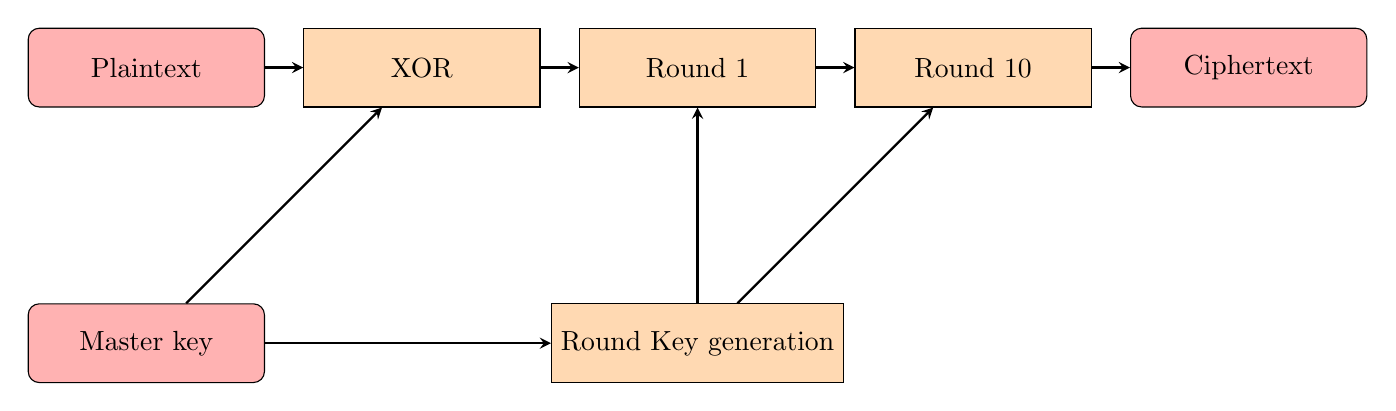
\begin{tikzpicture}[node distance=2cm ]
\node (plaintext) [startstop] {Plaintext};
\node (masterkey) [startstop, below of = plaintext, yshift=-1.5cm] {Master key};
\node (XOR) [process, right of = plaintext, xshift=1.5cm] {XOR};
\node (Roundfirst) [process, right of = XOR, xshift=1.5cm] {Round 1};
\node (Roundlast) [process, right of = Roundfirst, xshift=1.5cm] {Round 10};
\node (Ciphertext) [startstop, right of = Roundlast, xshift=1.5cm] {Ciphertext};
\node (RoundKey) [process, below of = Roundfirst, yshift=-1.5cm] {Round Key generation};
\draw [arrow] (plaintext) -- (XOR);
\draw [arrow] (XOR) -- (Roundfirst);
\draw [arrow] (Roundfirst) -- (Roundlast);
\draw [arrow] (Roundlast) -- (Ciphertext);
\draw [arrow] (masterkey) -- (RoundKey);
\draw [arrow] (masterkey) -- (XOR);
\draw [arrow] (RoundKey) -- (Roundfirst);
\draw [arrow] (RoundKey) -- (Roundlast);
\end{tikzpicture}
\end{adjustbox}
\end{frame}

\subsection{Rounds}

\begin{frame}
\frametitle{AES: Rounds}

\begin{adjustbox}{max totalsize={.9\textwidth}{.7\textheight},center}
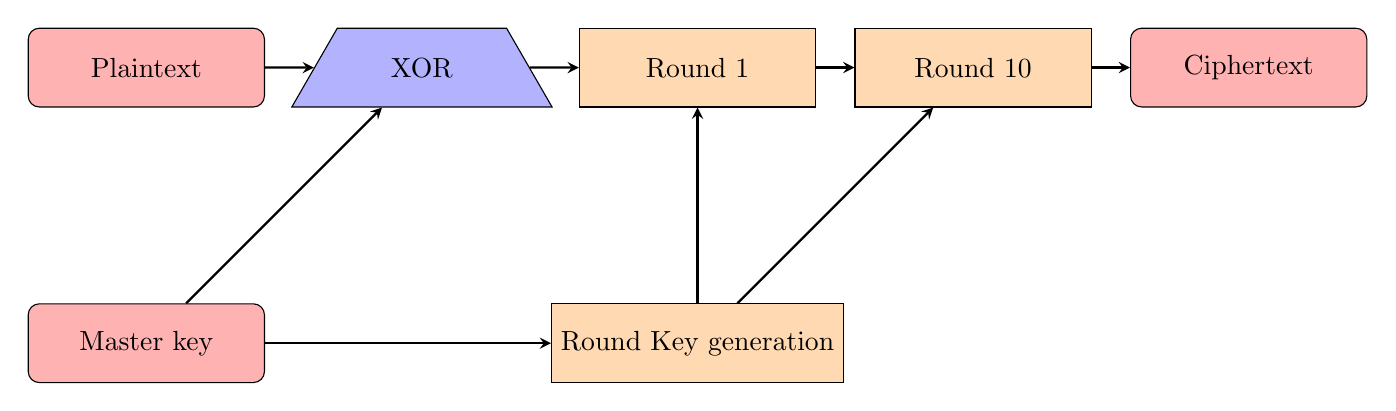
\begin{tikzpicture}[node distance=2cm]
\node (plaintext) [startstop] {Plaintext};
\node (masterkey) [startstop, below of = plaintext, yshift=-1.5cm] {Master key};
\node (XOR) [io, right of = plaintext, xshift=1.5cm] {XOR};
\node (Roundfirst) [process, right of = XOR, xshift=1.5cm] {Round 1};
\node (Roundlast) [process, right of = Roundfirst, xshift=1.5cm] {Round 10};
\node (Ciphertext) [startstop, right of = Roundlast, xshift=1.5cm] {Ciphertext};
\node (RoundKey) [process, below of = Roundfirst, yshift=-1.5cm] {Round Key generation};
\draw [arrow] (plaintext) -- (XOR);
\draw [arrow] (XOR) -- (Roundfirst);
\draw [arrow] (Roundfirst) -- (Roundlast);
\draw [arrow] (Roundlast) -- (Ciphertext);
\draw [arrow] (masterkey) -- (RoundKey);
\draw [arrow] (masterkey) -- (XOR);
\draw [arrow] (RoundKey) -- (Roundfirst);
\draw [arrow] (RoundKey) -- (Roundlast);
\end{tikzpicture}
\end{adjustbox}

\[
\pause \left( \begin{array}{cccc}
1 & 0 & 1 & 0 \\[0pt]
\bigoplus & \bigoplus & \bigoplus & \bigoplus \\[0pt]
0 & 1 & 1 & 0 \\[0pt]
= & = & = & = \\[0pt]
1 & 1 & 0 & 0 \\[0pt]
\end{array} \right)
\]

\begin{itemize}
\pause
\item bitwise logical operation; can be performed directly by the CPU \pause
\item addition mod 2 \pause
\item can randomize biased input
\end{itemize}
\end{frame}

\begin{frame}
\frametitle{AES: Rounds}
\begin{adjustbox}{max totalsize={.9\textwidth}{.7\textheight},center}
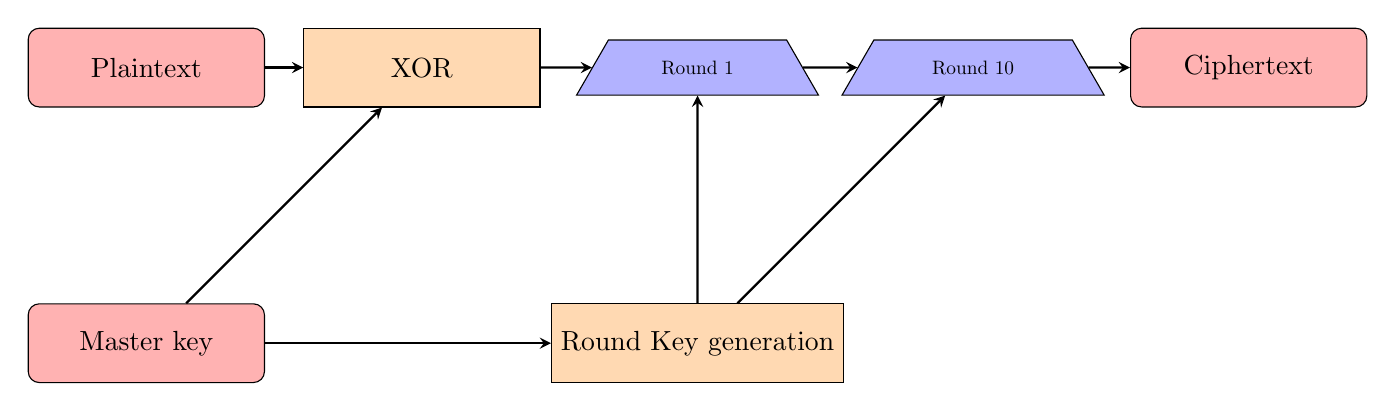
\begin{tikzpicture}[node distance=2cm]
\node (plaintext) [startstop] {Plaintext};
\node (masterkey) [startstop, below of = plaintext, yshift=-1.5cm] {Master key};
\node (XOR) [process, right of = plaintext, xshift=1.5cm] {XOR};
\node (Roundfirst) [io, right of = XOR, xshift=1.5cm, scale=0.7] {Round 1};
\node (Roundlast) [io, right of = Roundfirst, xshift=1.5cm, scale=0.7] {Round 10};
\node (Ciphertext) [startstop, right of = Roundlast, xshift=1.5cm] {Ciphertext};
\node (RoundKey) [process, below of = Roundfirst, yshift=-1.5cm] {Round Key generation};
\draw [arrow] (plaintext) -- (XOR);
\draw [arrow] (XOR) -- (Roundfirst);
\draw [arrow] (Roundfirst) -- (Roundlast);
\draw [arrow] (Roundlast) -- (Ciphertext);
\draw [arrow] (masterkey) -- (RoundKey);
\draw [arrow] (masterkey) -- (XOR);
\draw [arrow] (RoundKey) -- (Roundfirst);
\draw [arrow] (RoundKey) -- (Roundlast);
\end{tikzpicture}
\end{adjustbox}
\end{frame}

\begin{frame}
\frametitle{AES: Rounds}
\begin{adjustbox}{max totalsize={.9\textwidth}{.7\textheight},center}
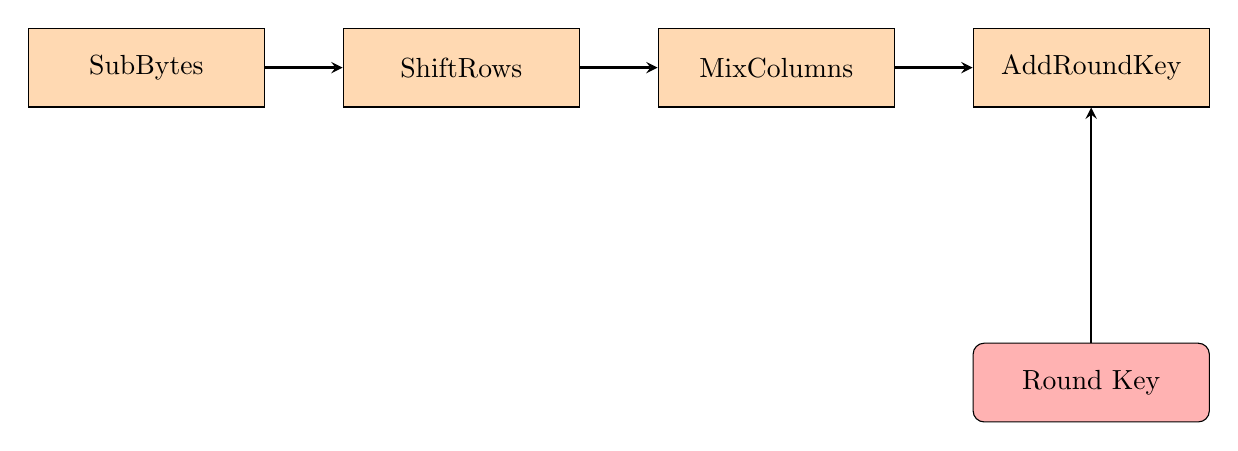
\begin{tikzpicture}[node distance=4cm]
\node (subbytes) [process] {SubBytes};
\node (ShiftRows) [process, right of = subbytes] {ShiftRows};
\node (MixColumns) [process, right of = ShiftRows] {MixColumns};
\node (AddRoundKey) [process, right of = MixColumns] {AddRoundKey};
\node (RoundKey) [startstop, below of = AddRoundKey] {Round Key};
\draw [arrow] (subbytes) -- (ShiftRows);
\draw [arrow] (ShiftRows) -- (MixColumns);
\draw [arrow] (MixColumns) -- (AddRoundKey);
\draw [arrow] (RoundKey) -- (AddRoundKey);
\end{tikzpicture}
\end{adjustbox}
\end{frame}

\begin{frame}
\frametitle{AES: SubBytes}
\begin{center}
\includegraphics<1>[scale=0.45]{SBox.PNG}
\end{center}
\begin{itemize}
\item<2-> Bytewise operation
\item<3-> Sole source of Confusion; the only non-linear operation in AES (affine transformation)
\item<4-> Key-independence is accepted in return for non-linearity; this eliminates one of DES' major weaknesses
\item<5-> Utilization of the multiplicative inverse maximizes non-linearity, but negatively impacts diffusion: $0^{-1} = 0$ and $1^{-1}=1$
\end{itemize}
\end{frame}

\begin{frame}
\frametitle{AES: ShiftRows}

\[ \left( \begin{array}{cccc}
a_{0,0} & a_{0,1} & a_{0,2} & a_{0,3} \\[0pt]
a_{1,0} & a_{1,1} & a_{1,2} & a_{1,3} \\[0pt]
a_{2,0} & a_{2,1} & a_{2,2} & a_{2,3} \\[0pt]
a_{3,0} & a_{3,1} & a_{3,2} & a_{3,3}\end{array} \right)
\xrightarrow{\text{ShiftRows}}
\left( \begin{array}{cccc}
a_{0,0} & a_{0,1} & a_{0,2} & a_{0,3} \\[0pt]
a_{1,1} & a_{1,2} & a_{1,3} & a_{1,0} \\[0pt]
a_{2,2} & a_{2,3} & a_{2,0} & a_{2,1} \\[0pt]
a_{3,3} & a_{3,0} & a_{3,1} & a_{3,2}\end{array} \right)
\]

\pause

\begin{itemize}
\item One of the two primary sources of diffusion \pause
\item One small change to the plaintext should result in a large change to the ciphertext \pause
\item Bytes are placed into the state in column order, but shifted across rows
\end{itemize}
\end{frame}

\begin{frame}
\frametitle{AES: MixColumns}

\[ \left( \begin{array}{cccc}
02 & 03 & 01 & 01 \\
01 & 02 & 03 & 01 \\
01 & 01 & 02 & 03 \\
03 & 01 & 01 & 02\end{array} \right)
\cdot
\left( \begin{array}{c}
a_0 \\
a_1 \\
a_2 \\
a_3\end{array} \right)
=
\left( \begin{array}{c}
s_0 \\
s_1 \\
s_2 \\
s_3\end{array} \right)
\]

\begin{columns}
\begin{column}{0.5\textwidth}
\pause
\begin{center}
$
s_0 = {02}a_0+{03}a_1+{01}a_2+{01}a_3 \\[0pt]
s_1 = {01}a_0+{02}a_1+{03}a_2+{01}a_3 \\[0pt]
s_2 = {01}a_0+{01}a_1+{02}a_2+{03}a_3 \\[0pt]
s_3 = {03}a_0+{01}a_1+{01}a_2+{02}a_3 \\[0pt]
$
\end{center}
\end{column}
\begin{column}{0.5\textwidth}
\begin{itemize}
\pause
\item Each new byte is dependent on an entire column of four old bytes \pause
\item Second source of diffusion
\end{itemize}
\end{column}
\end{columns}
\end{frame}


\begin{frame}
\frametitle{AES: AddRoundKey}
\end{frame}

\section{A Historical Transition}

\begin{frame}
\frametitle{Historical Impact of Cryptography}
\end{frame}

\begin{frame}
\frametitle{Motivator for more Powerful Computing}
\end{frame}

\begin{frame}
\frametitle{Today's Issues}
\end{frame}

\begin{frame}
\frametitle{The Modern War}
\end{frame}

 

\end{document}